\chapter{Progress Report}

GitHub was used for version control and mapping progress. Screenshots were taken along the way which show the scene through various stages of development.

A screenshot of the git history is shown [https://github.com/ccasey300/CG_Project.git]:

\begin{figure}
    \centering
    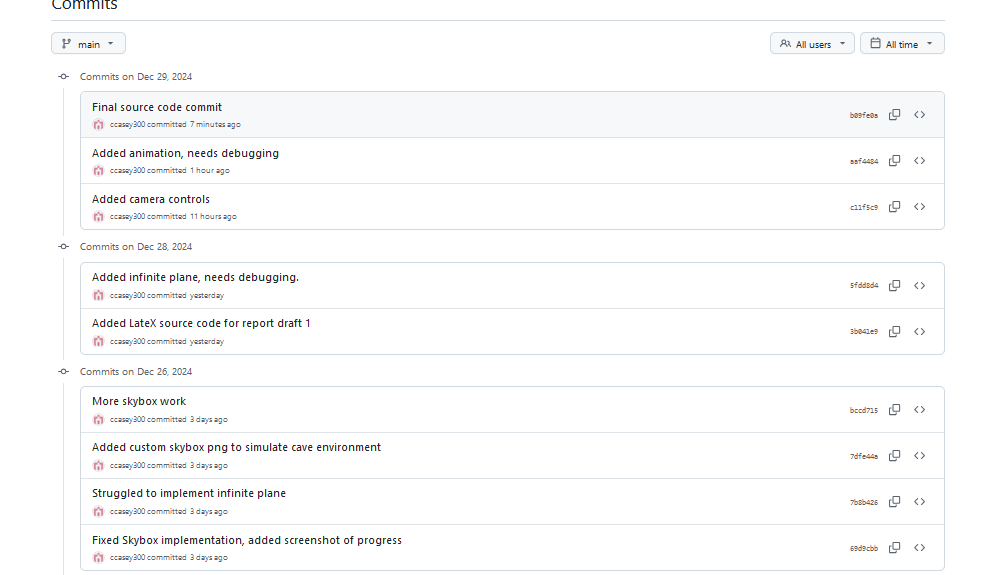
\includegraphics[width=0.5\linewidth]{Results//Progress_screenshots/Git History 2 (top of page)}
    \caption{This screenshot shows the  Git repository history (1/2).}
    %\label{fig:enter-label}
\end{figure}

\begin{figure}
    \centering
    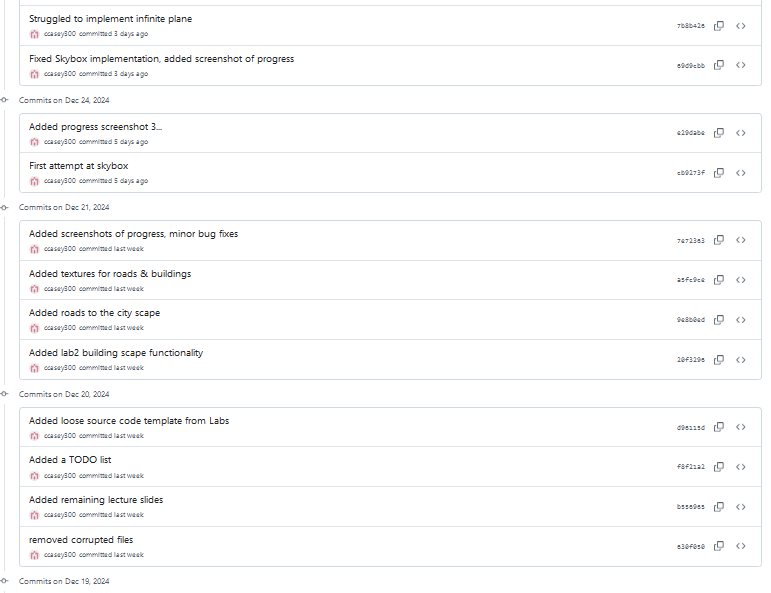
\includegraphics[width=0.5\linewidth]{Results//Progress_screenshots/Git History 1}
    \caption{This screenshot shows the  Git repository history (2/2).}
    %\label{fig:enter-label}
\end{figure}

\newpage
\section*{\Huge{Progress: Description of Screenshots}}

Screenshot 1: Geometry Rendering

Screenshot 2: Texturing and SkyBox

Screenshot 3: Custom SkyBox

Screenshot 4: Lighting and Shadows attempt

Screenshot 5: Animation attempt

Screenshot 6: Final Render


\newpage

\begin{figure}
    \centering
    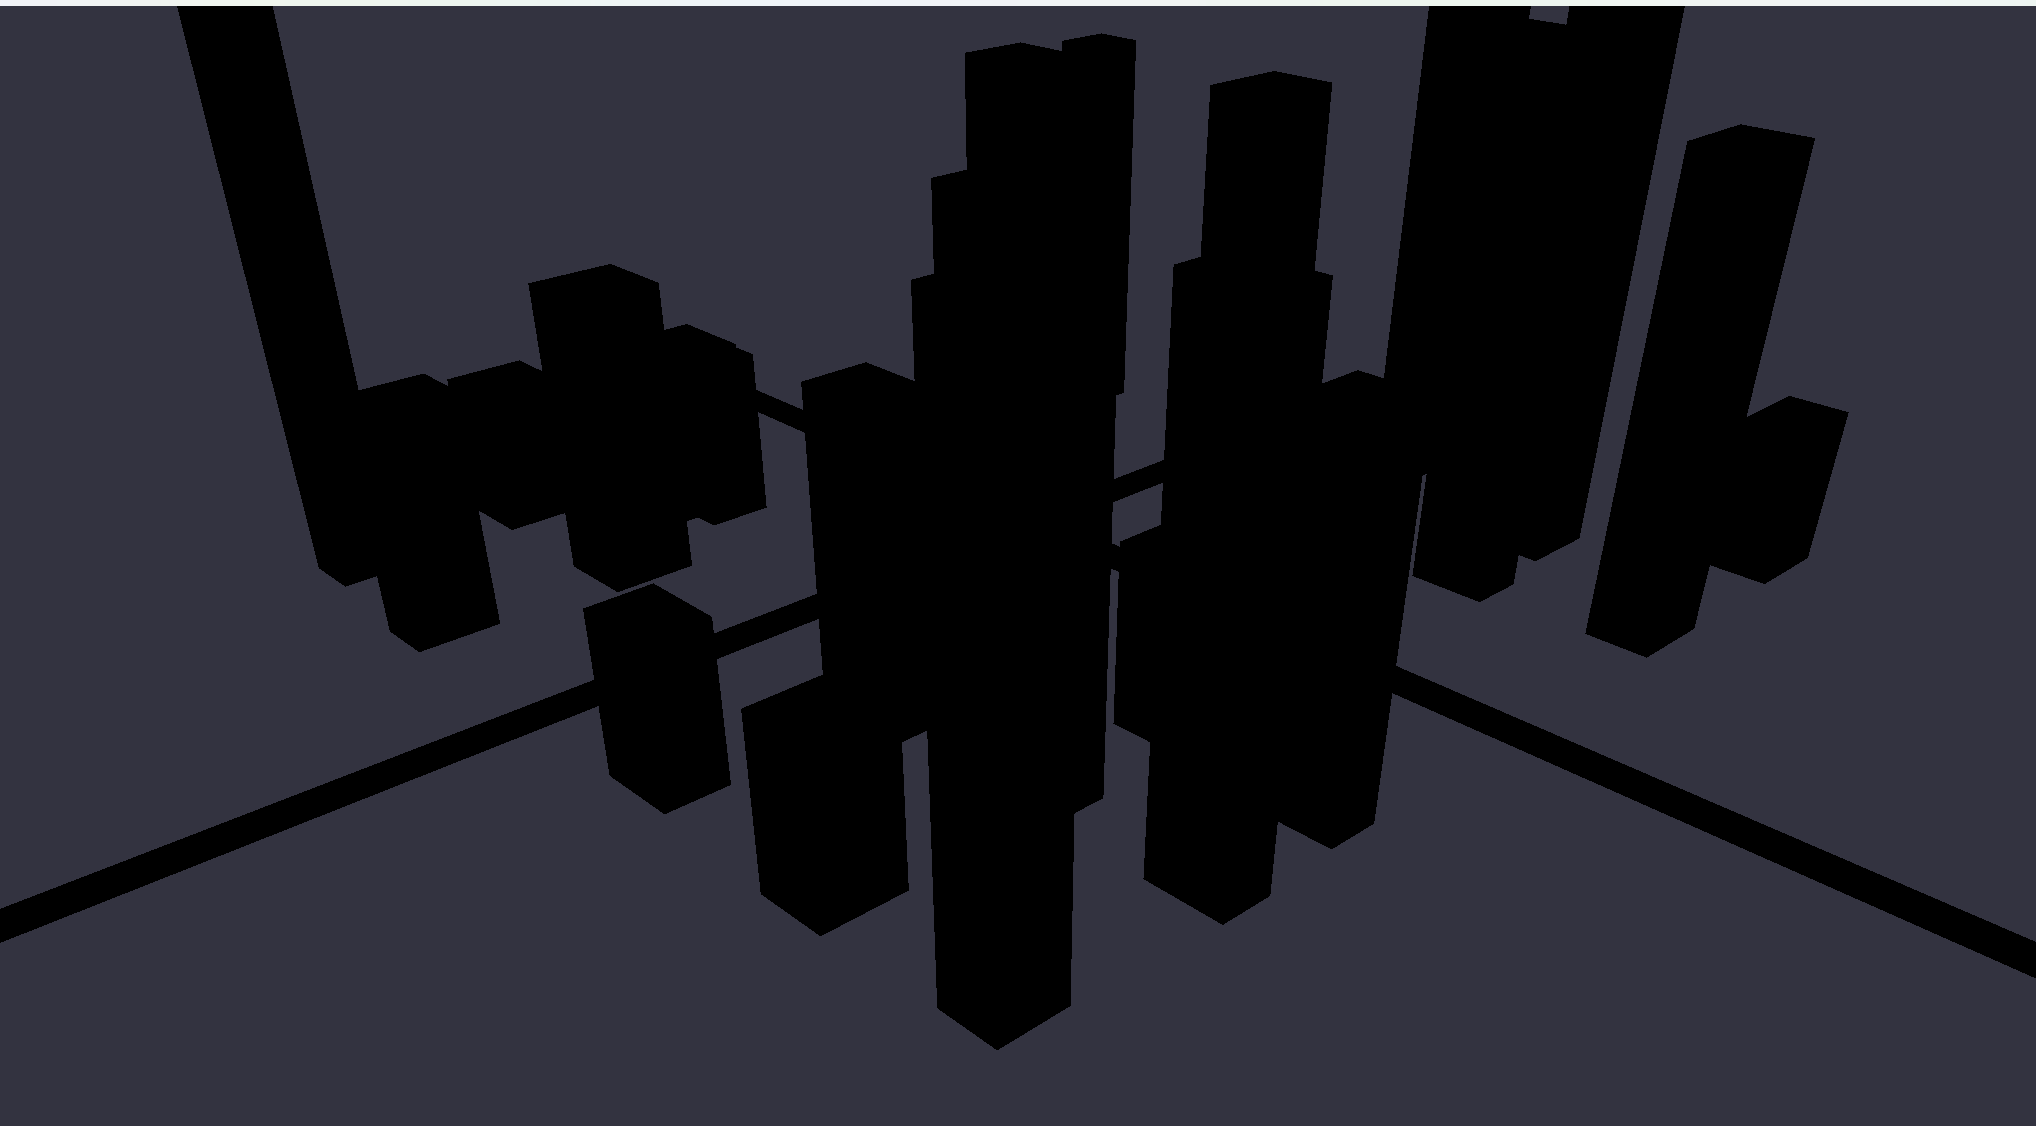
\includegraphics[width=0.5\linewidth]{Results//Progress_screenshots/Screenshot 1 - Geometry.png}
    \caption{This screenshot shows successful rendering of buildings and roads in the scene.}
    %\label{fig:enter-label}
\end{figure}
\begin{figure}
    \centering
    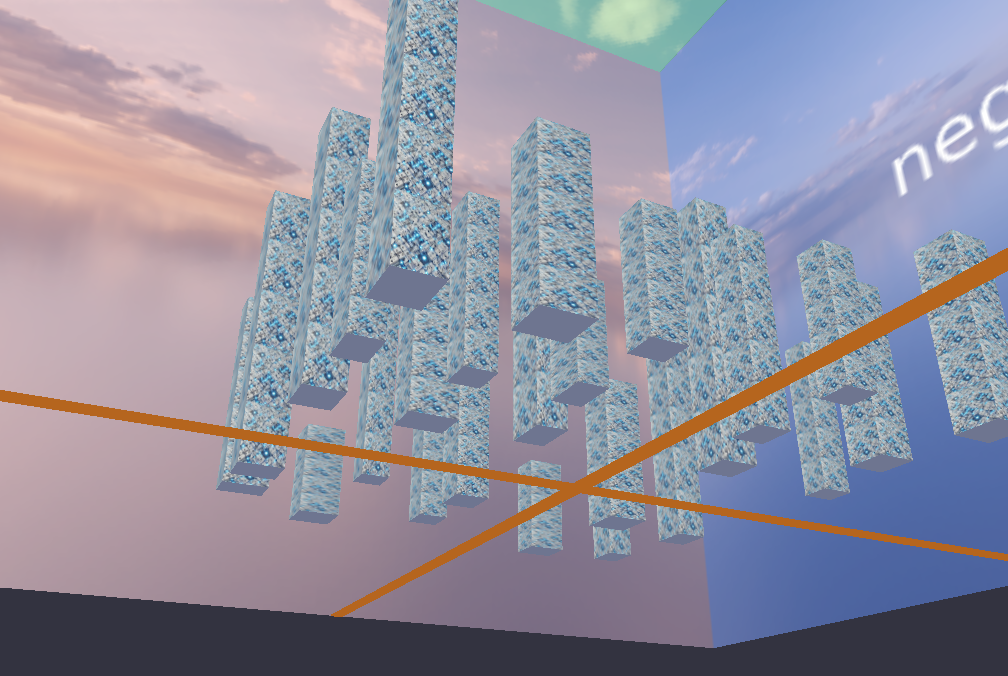
\includegraphics[width=0.5\linewidth]{Results//Progress_screenshots/Screenshot 3a - Skybox.png}
    \caption{This screenshot shows texturing of objects (buildings and roads), and implementation of skybox debug from lab 2.}
    %\label{fig:enter-label}
\end{figure}
\begin{figure}
    \centering
    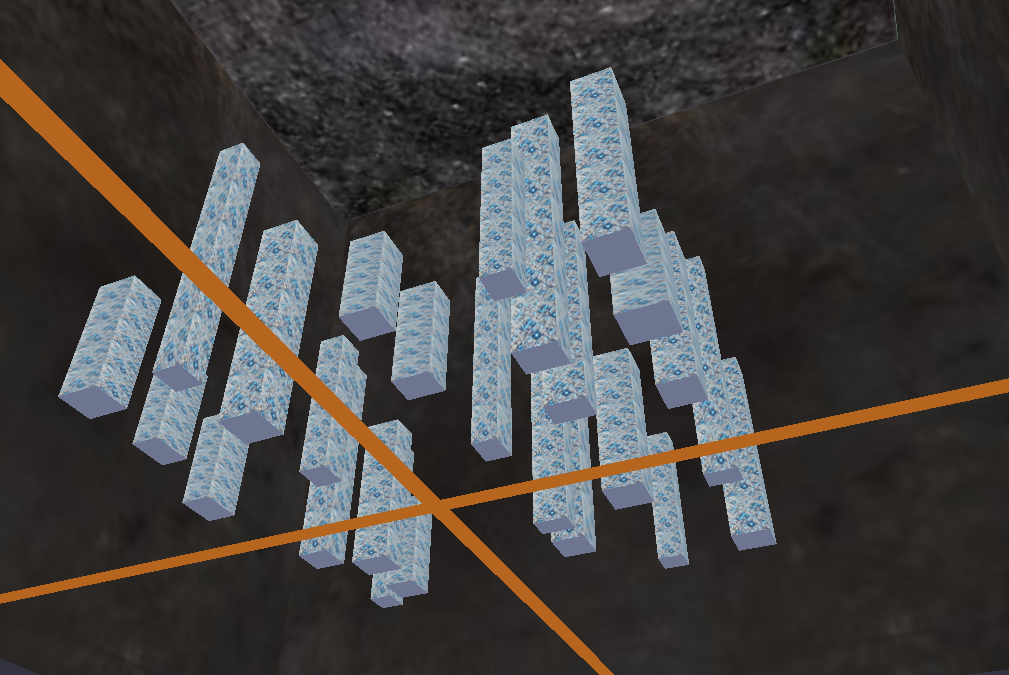
\includegraphics[width=0.5\linewidth]{Results//Progress_screenshots/Screenshot 3b - Custom Skybox.png.png}
    \caption{This screenshot shows a custom "cave themed" SkyBox. This was created using online resources like Adobe Image Editor and free-use google images.}
    %\label{fig:enter-label}
\end{figure}
\begin{figure}
    \centering
    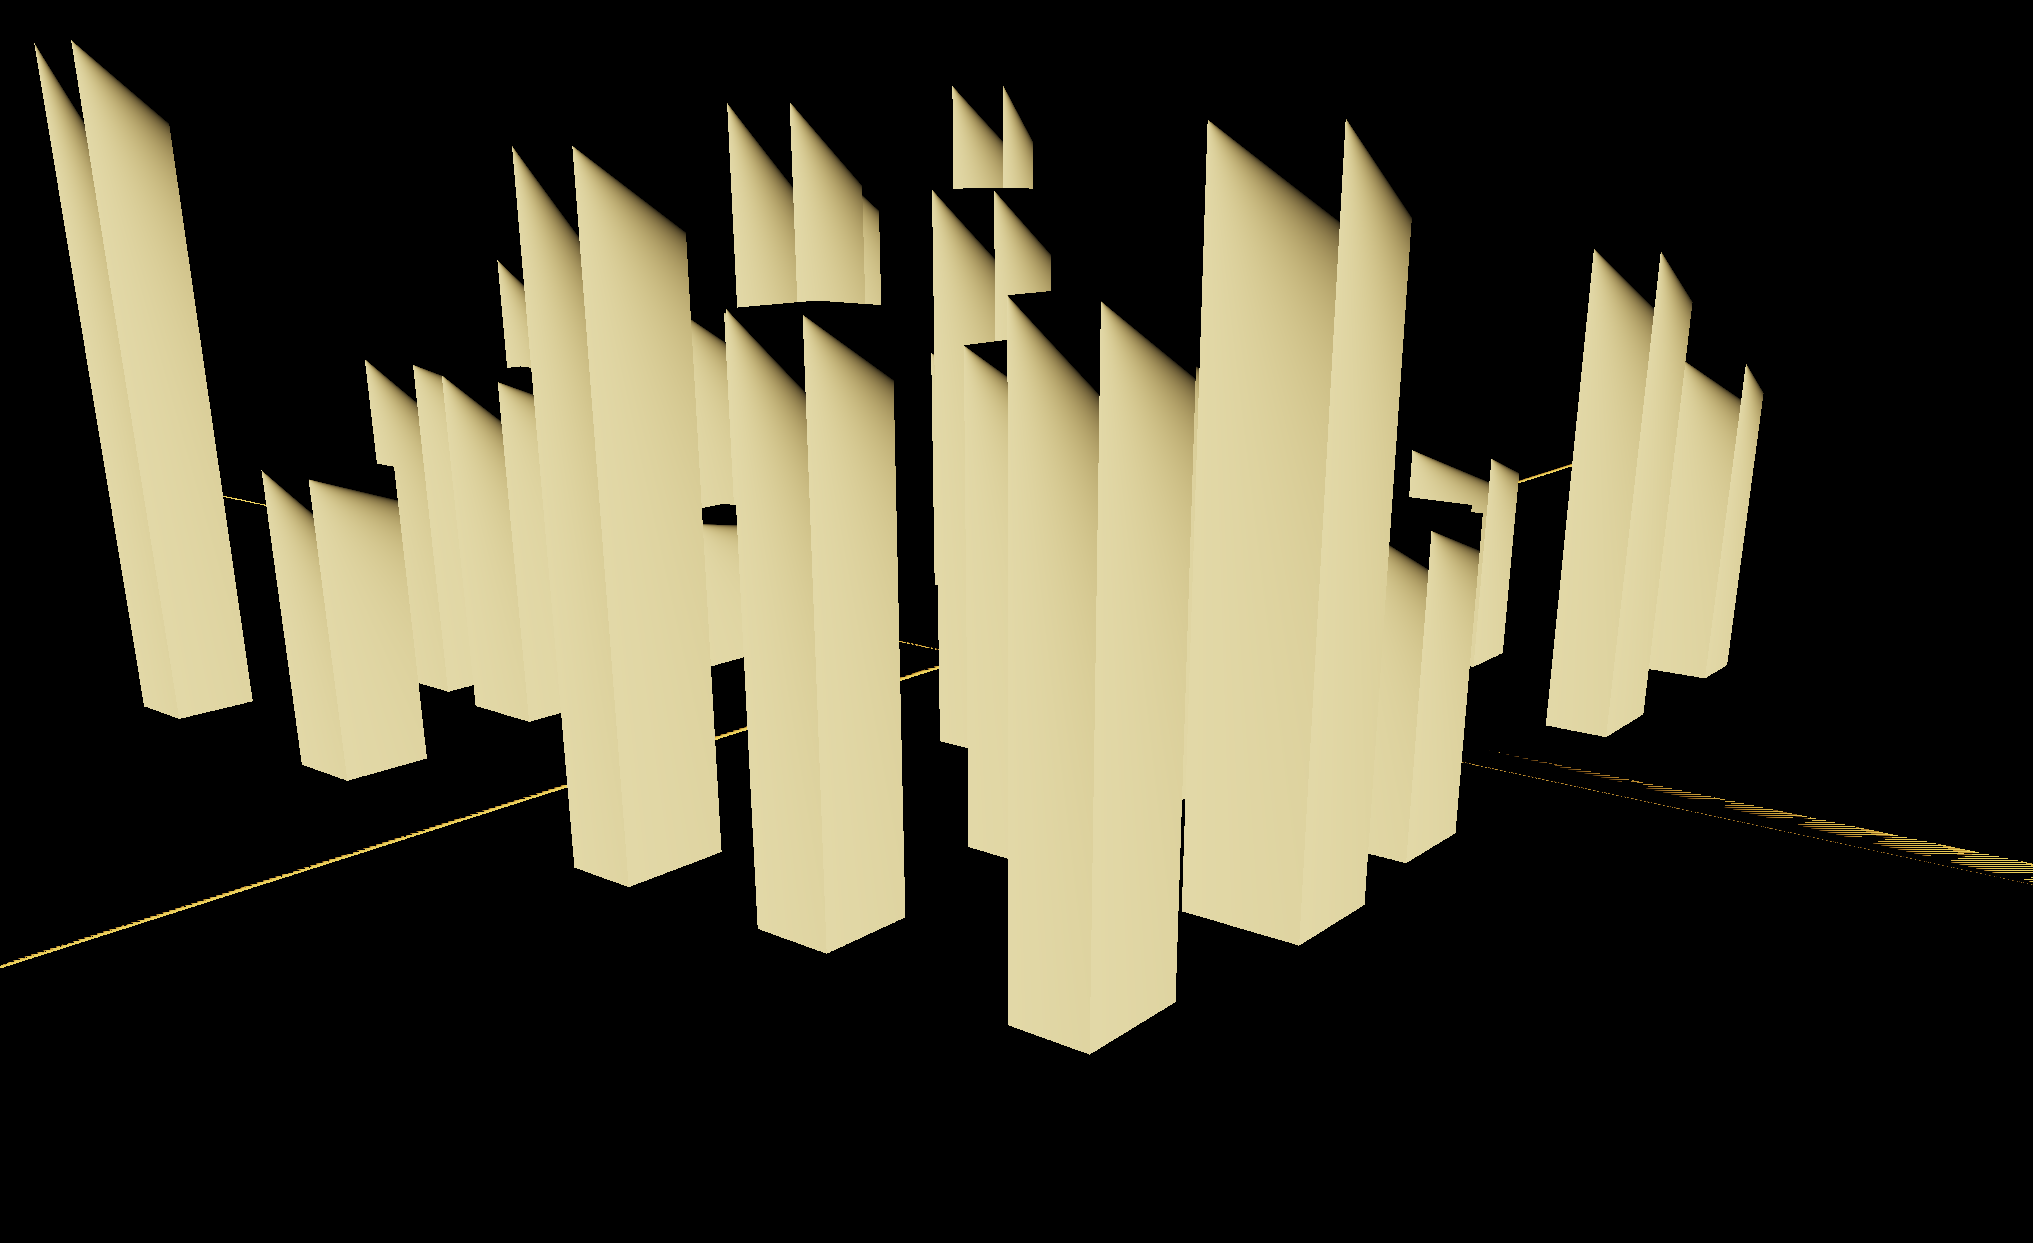
\includegraphics[width=0.5\linewidth]{Results//Progress_screenshots/Screenshot 4 - Lighting & Shadows Attempt.png}
    \caption{My attempt at lighting and shadows, progress can be seen but ultimately could not integrate with textures.}
    \label{fig:enter-label}
\end{figure}
\begin{figure}
    \centering
    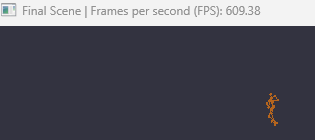
\includegraphics[width=0.5\linewidth]{Results//Progress_screenshots/Screenshot 5 - Animation}
    \caption{My attempt at including animation, could not resolve OGL parameter logic in time}
    \label{fig:enter-label}
\end{figure}
\begin{figure}
    \centering
    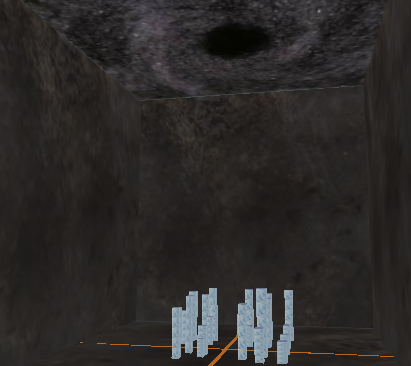
\includegraphics[width=0.5\linewidth]{Results//Progress_screenshots/Screenshot 6 - Final Render}
    \caption{Final render of scene}
    \label{fig:enter-label}
\end{figure}


\newpage
\chapter{Discussion: Quality + Robustness}
I primarily worked using a combination of different lab templates. I primarily used lab 2 and lab 4. However, this approach came with its limitations. Primarily, a lack of object-oriented code as well as being more application specific than I wanted. This lead to lengthy attempts and difficulty debugging. 

As a result, though the code is (maybe) easily understood upon visual inspection, additional elements required a significant amount of work in order to integrate with the existing scene. In this way, I was too dependent on the templates given and should have deviated my approach earlier.

There is some redundant code, several similar structs were defined in order to resolve some texturing issues I faced. If I had more time in the future I would take the existing functionality and try to leverage OOP.



The code includes error-handling much in the same way we did in class. File loading, shader implementation and null pointers are managed appropriately. All cleanup is done after rendering as required. Performance was consistently good, however was never properly challenged. The option to include more animation, more lighting, etc. is there. The scene consistently runs well over 15 FPS on my laptop.